%%
%% Beuth Hochschule für Technik --  
%%
%% Kapitel 3 - Desktop App
%%
%%	

\chapter{Desktop App}
Zu der Android App gibt es parallel eine App für den Desktop. Diese wurde mit JavaFX  programmiert. In den folgenden Kapiteln wird die ungefähre Programmierung der einzelnen Stages beschrieben.

\lstset{language=Java,
				backgroundcolor=\color{light-gray},
				%frame=single,
				tabsize=2,
				breaklines=true,
				%numbers=left,
				numbersep=5pt,
				%numberstyle=\color{light-gray},
				basicstyle=\ttfamily\color{black}\small,
				keywordstyle=\color{HKS51}\bfseries,
				commentstyle=\color{HKS13}\slshape,,
				identifierstyle=\color{blue},
				stringstyle =\color{orange}}
				
				
\section{Was ist JavaFX ?}
JavaFX ist eine Java-Spezifikation, die als Hauptkonkurrenten Adobe Flash und Microsoft Silverlight hat. Ein positiver Punkt ist der Lauffähigkeit auf diversen Geräten wie z.B. Mobilfunk, Desktop-Computern, Embedded Geräten und Blu-ray Geräten. Die Programmierung findet ganz normal wie in Java statt. Die dazu gehörigen Bibliotheken werden seit der Java SE Runtime 7 Update 6 automatisch mitinstalliert. Es ist unter anderem auf die Grafikprogrammierung ausgelegt. Dadurch lassen sich grafische Elemente schnell programmieren und mit CSS gestalten.
Ein sehr bekanntes Embedded Gerät, wofür es auch JavaFX gibt, ist das Raspberry PI. \cite{bib.jFXRaspPi}

\section{Struktur und Aufbau der App}
Es gibt insgesamt fünf verschiedene Stages in der App.
\begin{itemize}
	\item Login (siehe \ref{subsec.login})
	\item Registrierung (siehe \ref{subsec.registrierung})
	\item Control (siehe \ref{subsec.control})
	\item Datenbank (siehe \ref{subsec.datenbank})
	\item Foto (siehe \ref{subsec.foto})
\end{itemize}

In JavaFX ist ein Fenster ein Stage-Objekt. Diesem Stage-Objekt können mehrere anderer Objekte hinzugefügt werden. Bei diesen anderen Objekten kann es sich um Buttons, eine Tabelle, ein Textfeld usw. handeln.

\begin{figure}[h]
  \begin{center}
    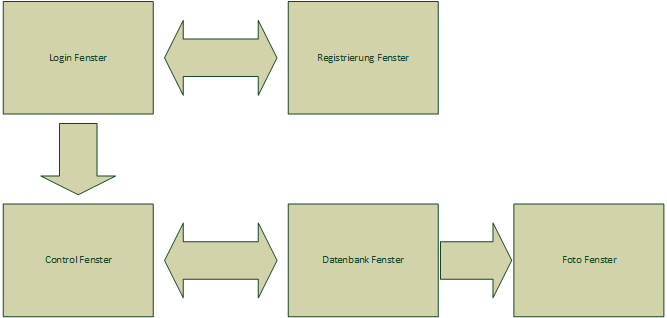
\includegraphics[scale=0.7]{MaskenDesktopVersion.png}
  		  \caption{Aufbau der App}
     \label{fig.MaskenDesktopVersion}
  \end{center}
\end{figure}\newpage

\subsection{Login}
\label{subsec.login}
Bei dem Login Fenster muss sich der Nutzer mit seinem Usernamen und Passwort, was in der Datenbank hinterlegt ist, anmelden. Ist einer der Felder nicht ausgefüllt oder das Passwort bzw. der User nicht korrekt, wird das mit einem \texttt{Label} als Message dargestellt. Über eine \texttt{CheckBox} kann der Benutzer sich sein Passwort in Klartext anzeigen oder verbergen lassen. Dies wurde so realisiert das ein \texttt{TextField} Objekt und ein \texttt{PasswordField} Objekt direkt übereinander gelegt wurden. Der Initialisierungszustand ist der, das das \texttt{PasswordField} sichtbar und das \texttt{TextField} unsichtbar ist. Mit der \texttt{CheckBox} wird das Ganze dann getoggelt.
\begin{lstlisting}[caption={Java Passwort-, Textfeld Un-, Sichtbar}\label{lst:reg.java.pw.txt},captionpos=b]
		pwTextField.managedProperty().bind(checkBox.selectedProperty());
		pwTextField.visibleProperty().bind(checkBox.selectedProperty());

		passwordField.managedProperty().bind(checkBox.selectedProperty().not());
		passwordField.visibleProperty().bind(checkBox.selectedProperty().not());
\end{lstlisting}
Damit das Eingegebene mit in dem anderen Feld erscheint, werden beide Felder bidirektional miteinander verbunden.
\begin{lstlisting}[caption={Java Passwort-, Textfeld bidirektional}\label{lst:reg.java.bidirektional},captionpos=b]
		pwTextField.textProperty().bindBidirectional(
						passwordField.textProperty());
\end{lstlisting}
\begin{figure}[h]
  \begin{center}
    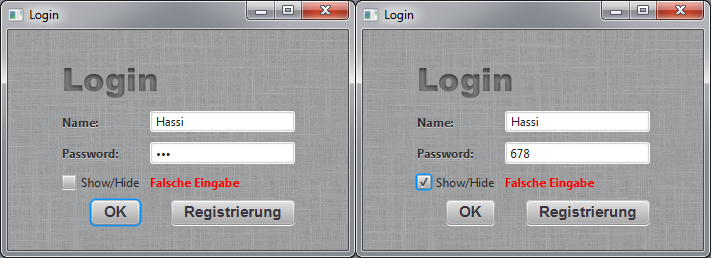
\includegraphics[scale=0.6]{loginStage.png}
  		  \caption{Login Fenster}
     \label{fig.loginFenster}
  \end{center}
\end{figure}

\subsection{Registrierung}
\label{subsec.registrierung}
Falls der Benutzer noch kein Konto in der Datenbanktabelle \texttt{tb\_Users} hat, hat er die Möglichkeit, sich über das Registrierungsfenster anzumelden. Softwareseitig wurde eine Überprüfung eingebaut, dass jedes Textfeld etwas beinhalten muss. Bei den Passwortfeldern wird überprüft, ob die beiden Passwörter, die eingegeben wurden, identisch sind. Wenn alle Überprüfungen korrekt sind, wird aus den Eingaben und einem SQL Befehl \texttt{NOW()} ein SQL-String gebaut und an die Datenbank geschickt. Falls die Überprüfung fehlgeschlagen ist, wird wie im  Login Fenster (s. \ref{subsec.login}) eine \texttt{Label} Message ausgegeben.
%%%%%%%%%%%%%%%%%%%%%%%%%%%%%%%%%%%%%%%%%%%%%%%%%%%%%%%%%%%%%%%%%%%%%%%%%%%
%referenz auf die DB wie sie aufgebaut ist ???
%%%%%%%%%%%%%%%%%%%%%%%%%%%%%%%%%%%%%%%%%%%%%%%%%%%%%%%%%%%%%%%%%%%%%%%%%%%
\begin{lstlisting}[caption={Java-SQL neuer Benutzer}\label{lst:reg.java.eintrag},captionpos=b]
	String SQL = "INSERT INTO tb_user VALUES (null,'"
									+ txtVorname.getText() + "', '"
									+ txtNachname.getText() + "', '"
									+ txtEmail.getText() + "', '"
									+ txtUserName.getText() + "', '"
									+ txtPw.getText() + "', NOW())";
\end{lstlisting}
Der folgende String zeigt die Darstellung, wie der obige String mit Nutzerdaten aussieht und an die Datenbank gesendet wird.
\begin{lstlisting}[caption={SQL Beispiel String}\label{lst:reg.sql.eintrag},captionpos=b]
	INSERT INTO tb_user VALUES (null,'Gernot', 'Hassknecht', 'heutShow@zdf.de',
			 'Hassi', '007', NOW())
\end{lstlisting}

Der Befehl \texttt{NOW()} wird in der Datenbank mit dem aktuellen Datum und Uhrzeit ersetzt.
Die Sichtbarkeit der Anmeldedaten ist nur direkt innerhalb der Applikation möglich. In diesem Fall mit einem System.out.println() in Eclipse. Was nicht mehr weiter implementiert wurde, ist eine zusätzliche Freischaltung des neuen Users von einem Admin. Nach direkter Registrierung kann sich der User sofort anmelden.
\begin{figure}[h]
  \begin{center}
    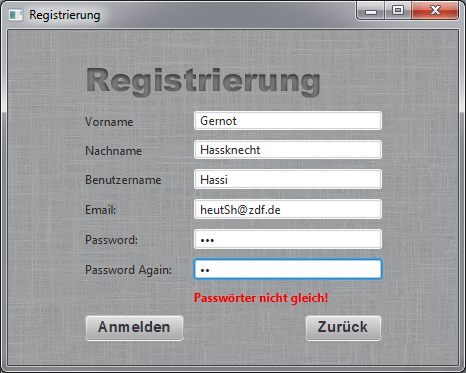
\includegraphics[scale=0.6]{regStage.png}
  		  \caption{Registrierung Fenster}
     \label{fig.RegistrierungFenster}
  \end{center}
\end{figure}

\subsection{Control}
\label{subsec.control}

Im Fenster \texttt{Control} ist es möglich, das Live-Video von der Cam zu betrachten. Es wird mit Hilfe der Klasse WebEngine und WebView realisiert. D.h. es wird durch WebEngine die Webseite geladen und durch WebView wird die geladene Webseite im Fenster angezeigt. Diese Webseite wird vom MJPEG Streamer zur Verfügung gestellt. Der Stream wird erst gestartet, wenn das Fenster \texttt{Control} geöffnet ist.

\begin{lstlisting}[caption={Stream Einbindung}\label{lst:reg.java.stream},captionpos=b]
WebView webview = new WebView();
webview.setVisible(true);
WebEngine webengine = webview.getEngine();
webengine.setJavaScriptEnabled(true);
File file = new File("http://<IP-Adresse vom PI>/javascript\_simple.html");
webengine.load(file.toString());
\end{lstlisting}

Beim Betätigen des Buttons \texttt{Database} wird ein neues Fenster \texttt{Datenbank} geöffnet (siehe Kapital \ref{subsec.datenbank}) und das Fenster \texttt{Control} wird geschlossen. 
Nach dem Betätigen des Buttons \texttt{Open} werden zwei Funktionen aufgerufen. Bei der ersten Funktion wird mit einem HTTP-POST ein Befehl an das PI gesendet, das dieses die Tür öffnen kann. Bei der zweiten Funktion wird ein neuer Eintrag in die Tabelle \texttt{tb\_doorloogers} in Datenbank eingetragen. Dieser Eintrag beinhaltet den Zeitpunkt des Öffnens der Tür.


\begin{figure}[h]
  \begin{center}
    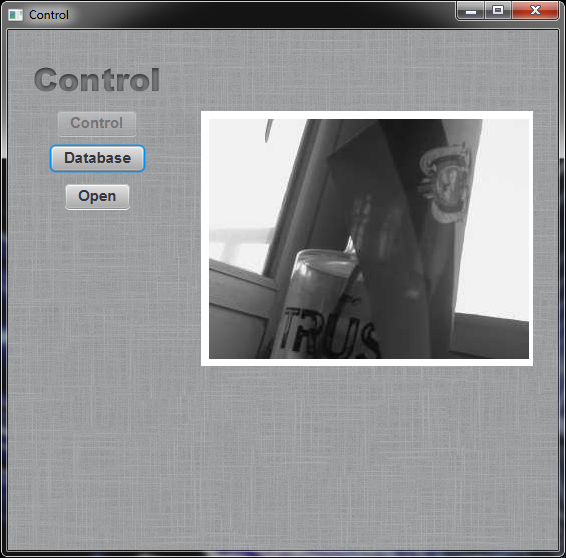
\includegraphics[scale=0.5]{streamStage.png}
  		  \caption{Control Fenster}
     \label{fig.StreamFenster}
  \end{center}
\end{figure}

\subsection{Datenbank}
\label{subsec.datenbank}
Diese Stage hat als Hauptobjekt eine Tabelle. Der Tabelleninhalt wird dynamisch erstellt. In einer zusätzliche Klasse wird geschaut, wie viele Spalten die Datenbank hat und fügt diese dann dem Tabellen-Objekt hinzu. Nach dem Hinzufügen der Spalten wird Zeile für Zeile aus der Datenbank geholt und in die Tabelle geladen. Zu jedem Eintrag in die Datenbanktabelle \texttt{tb\_doorlogger} gehört ein Bild. Um sich zu einen entsprechenden Tabelleneintrag das Bild anzusehen, muss man über eine Combobox die ID der Zeile auswählen und auf den Button \texttt{Open Picture} klicken. Mehr dazu im Kapitel \ref{subsec.foto}. Die Combobox zeigt nur so viele Zahlen wie es Zeilen in der Tabelle gibt. Wenn nichts in der Datenbank steht und dadurch auch kein Eintrag in die Tabelle gemacht wird, werden die Combobox und der \texttt{Open Picture} Button deaktiviert. Gibt es Einträge in der Datenbank, so ist die Standarteinstellung der Combobox auf 1.

\begin{figure}[h]
  \begin{center}
    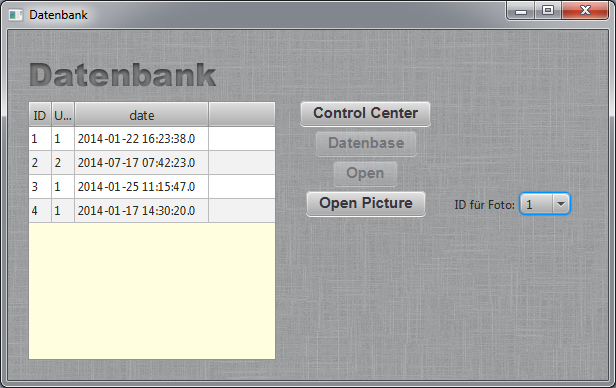
\includegraphics[scale=0.6]{dbStage.png}
  		  \caption{Datenbank Fenster}
     \label{fig.DatenbankFenster}
  \end{center}
\end{figure}

\subsection{Foto}
\label{subsec.foto}
Nachdem der \texttt{Open Picture} Button in der Datenbank Ansicht gedruckt wurde, wird mit Hilfe der angegebenen ID aus der Combobox der SQL-String gebaut.

\begin{lstlisting}[caption={Java-SQL String Foto öffnen}\label{lst:pic.db.foto.open},captionpos=b]
String SQL = "SELECT * FROM tb_images WHERE ID = " + userID;
\end{lstlisting}

Aus dem String ist relativ leicht zu erkennen, dass das Bild aus der Datenbanktabelle \texttt{tb\_images} kommt. Das Bild ist aber in der Datenbank nur binär als BLOB Typ abgelegt. Dieser Typ existiert auch in Java. Nach dem Auslesen des Binärstreams wandeln wir das Gelesene in ein Byte-Array. Aus dem Byte-Array erzeugen wir dann ein Buffered-Image. In Swing könnten wir uns jetzt schon ein Bild anzeigen lassen. Aber das Programm wurde ja nicht mit Swing, sondern mit JavaFX geschrieben. Dank eines \texttt{.toFXImage(BufferedImage arg0, WritableImage arg1)} Befehles lässt sich unser Swing-Objekt einfach in ein JavaFX-Objekt umwandeln. Dieses zeigen wir dann in einem zusätzlichen Stage Fenster an. Ein klarer Vorteil bei dieser Methode ist, dass es nicht wichtig ist, was für ein Typ dem Bild mal angehörte.
\begin{lstlisting}[caption={JavaFX Foto öffnen}\label{lst:pic.javafx.open},captionpos=b]
//Foto aus DB holen
byte[] imgData = imgShow.getImageDB(userID);
...
//Foto nach JavaFX Objekt wandeln
SwingFXUtils.toFXImage(bufImg, img2);

//Foto imageView hinzufügen
imageView.setImage(img2);
\end{lstlisting}

\section{Problematik der Verwaltung der Fenster}
Während der Entwicklung der Desktop Applikation in JavaFX gab es technische Schwierigkeiten mit der Schließung der einzelnen Fenster. Wenn im Fenster ein Button betätigt wird, der gleichzeitig ein neues Fenster öffnen und das aktuelle Fenster schließen soll, wird ungewollt der gesamte Java-Applikation Prozess gekillt. Besonders bei dem Fenster mit dem Stream gab es ein weiteres Problem, dass nach der Schließung des Stream-Fensters der Stream im Hintergrund weiterlief. Es muss ein Konzept zur korrekten Schließung der Fenster erstellt werden, sodass eine Window-Klasse die einzelnen Fenster zur Öffnung und Schließung steuert. Das Konzept wurde zum Teil aus Zeitgründen nicht vollständig umgesetzt. Die Umsetzung wurde jetzt so realisiert, dass das aktuelle Fenster zuerst das kommende Fenster aufruft, dann wird erst das aktuelle Fenster geschlossen. Bei dem Fenster mit dem Stream wurde nicht mit der Klasse \texttt{MediaView} sowie \texttt{MediaPlayer} gearbeitet, sondern mit der Klasse \texttt{webView} und \texttt{webEngine}. Damit konnte auch das Problem mit dem ungewollten Weiterlaufen des Streams im Hintergrund gelöst werden.